\chapter{Contributions}\label{contributions}

\todo[inline]{Revision 2:\\-updated description of contributions}

The contributions of this PhD work are presented according to four
areas. The contribution of my PhD work are:

\begin{enumerate}
\def\labelenumi{\arabic{enumi}.}
\itemsep1pt\parskip0pt\parsep0pt
\item
  Implementation and evaluation of MIRROR Computer Supported Reflective
  Learning (CSRL) theory
\item
  Knowledge about designing experience-capturing tools for crisis
  workers
\item
  Novel sensing-based interaction techniques to support re- creation and
  generation of work experiences in crisis training
\item
  Knowledge about implementing prototypes to be deployed into the wild
\end{enumerate}

Contributions 1 maps CSRL theory with technology thru a design science
research methodology, contribution 2 provided design challenges for the
technology tools created, contribution 3 relates to the design of novel
interaction techniques to fit case studies requirements. Finally
contribution 4 shades the light on challenges in building prototypes to
implement the design.

\section{C1: Implementation and evaluation of MIRROR Computer Supported
Reflective Learning (CSRL)
theory}\label{c1-implementation-and-evaluation-of-mirror-computer-supported-reflective-learning-csrl-theory}

Contribution 1 of the thesis comprises new knowledge about how
theoretical concepts in the CSRL model can be mapped to technologies and
implemented in artefacts. The work provided successful applications of
technologies, in crisis training, that constitute an empirical
evaluation of the model itself.

The CSRL model developed by Krogstie et al. \autocite*{Krogstie:2013kf}
(Figure \ref{fig:csrl-model-contrib})and summarised in Chapter
\ref{csrl} presents a cycle of four stages to conceptualise reflection
at work. For each stage a set of reflection-useful activities that can
be enhanced by technology are presented. During this PhD work two of the
four stages of the model,\emph{plan and do work} and \emph{conduct
reflection session}, have been instantiated and specific activities from
each stage have been supported technology tools.
\todo{add a table with csrl phases - technology mapping}

\begin{figure}[tbh]
    \centering
    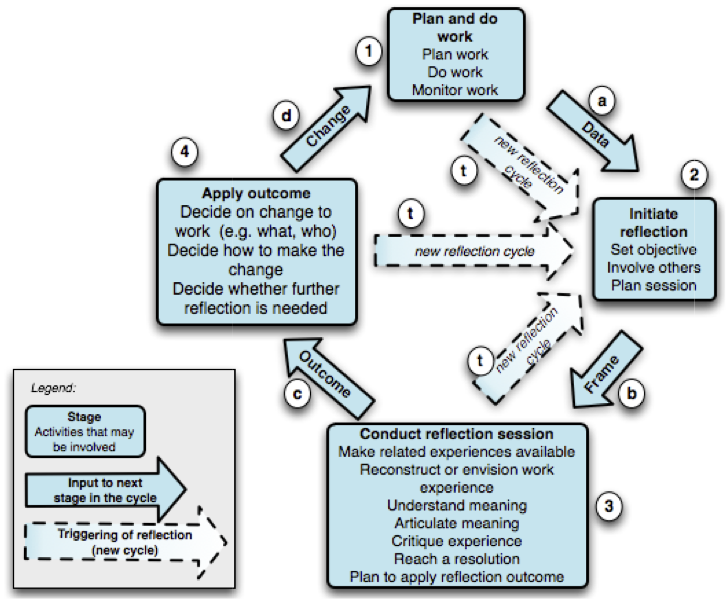
\includegraphics[width=1\textwidth]{CSRL}
    \caption{CSRL reflection cycle. Figure adapted from \protect\autocite{Krogstie:2013kf}}
    \label{fig:csrl-model-contrib}
\end{figure}

During \emph{plan and do work} the \emph{monitor work} and \emph{do
work} activities have been supported. The \emph{monitor work} activity
has been implemented by WATCHiT (P3) which empowers workers for
capturing a wide spectrum of qualitative and quantitative data. I found
out that \textbf{wearable sensor technology and embodied user
interfaces} provided the best design choice for data collection. The
\emph{do work} activity has been supported by Don't Panic (P4,P5), by
generating realistic work experiences that push workers towards taking
actions common of real work and under stress conditions. Although the
\emph{do work} phase in the model describes real work activities, for
the specific case of crisis management we claim it can also be applied
to simulated work. Indeed, It has been found out that the innovative
\textbf{digital board game technology} presented in P5 was effective in
recreating stress conditions similar to real work and collaboration
affordances typical tho the ones observed in a crisis decision room.

During \emph{Conduct reflection session} CroMAR (P1) supports a wide
range of activities. First it makes \emph{related experiences available}
by aggregating data about from multiple sources, including work
experience of colleagues (captured by WATCHiT), social networks and open
data. Then CroMAR allows to visualise data while being situated in a
physical context that helps \emph{reconstruct or envision work
experiences}. By allowing layering and filtering of data according to
source, time and space it facilitates \emph{understand and articulate
meanings}. Finally an embedded text editor allows for the collection and
sharing of lesson learnt and to elaborate a \emph{plan to apply
reflection outcomes}. Thanks to the experience with CroMAR we also found
out that \textbf{mobile augmented reality technology} is efficient in
supporting debriefing and reflection after crisis work.

Contribution 1 can be a resource for researcher in the field of computer
supported reflective learning that strives in finding solutions to map
theory tools to technology tools that people can use at work. Although
the applications developed are tailored to the crisis training domain,
they could be repurposed to other domains. The need for pervasive data
collection and disruption-free interfaces is shared by many work
practices; the digital board game approach developed in P5 has been
proven to be a useful tool also in generating realistic work experiences
for the dementia care domain, as investigated during research work
abroad (see Section ref\{context-of-the-work\}). Finally we demonstrated
a new application domain for mobile augmented reality technology: to
support debriefing. CroMAR, the tool we developed, could be adapted to
support debriefing of work practices that share similarities with the
crisis domain. The presented applications of technology constitute an
empirical evaluation of theory which outcomes (P2,P6) can inform future
development of the CSRL model. Finally a new approach to the design of
technology to turn unstructured context data into learning contents was
presented in P6 and evaluated across two cases studies. The approach
aims at extending the body of knowledge in computer-supported reflective
learning.

\section{C2: Knowledge about designing experience-capturing tools for
crisis
workers}\label{c2-knowledge-about-designing-experience-capturing-tools-for-crisis-workers}

Contribution 2 of this thesis is a set of challenges for the design of
technology tools for experience-collection during real or simulated
crises.

Seven design challenges, derived from multiple user studies with crisis
workers (summarised in Table \ref{field-studies}), have been reported in
P3. Despite there are guidelines for designing sensor and capturing
tools for a variety of domains; in this work I focused on capturing
information that is is relevant for crisis learning. The challenges shed
light on \emph{what} information is relevant and \emph{how} to capture
relevant information. This contribution also highlights a design
trade-off common for many sensing application: the degree of data that
can be captured with sensors, automatically and without user
intervention, versus information that can be submitted in-action by
workers themselves; which, in the case of crisis training, requires
novel interaction modalities (contribution 3). With the former being
fine-granular quantitative data, and the latter qualitative
semantically-rich information.

The challenges have informed the design of WATCHiT, a modular data
capturing tool (P3) that has been successfully evaluated in a scenario
to support debriefing after procedural training (P2). WATCHiT can be
configured to address new scenarios, data captured can be used to
support coordination of work or monitoring activities in real time.

Contribution 2 can be a resource for computer scientists aiming at
designing technologies for pervasive, quantitative and qualitative data
collection. The presented challenges constitute a foundation for a
design space for data capturing tools. They are expression of the
trade-off between technology-centred quantitative data acquisition and
user-centerer qualitative information collection.

\section{C3: Novel sensing-based interaction techniques to support
recreation and generation of work experiences in crisis
training}\label{c3-novel-sensing-based-interaction-techniques-to-support-recreation-and-generation-of-work-experiences-in-crisis-training}

Contribution 3 of the thesis brings novel interaction techniques to the
field of sensing-based interfaces.

The interaction techniques developed assist different tasks.

During \emph{capturing work experiences} the focus is on empowering
users for collecting work experiences without disrupting the work due to
interaction with the capturing tool. Building on prior works on mnemonic
shortcuts and body-centric interaction in P3 a novel disruption-free
user interface is presented. It allows to use predefined body areas and
objects as mnemonic shortcuts to activate sensors and to tag
quantitative data with user-submitted information.

To enhance \emph{re-creating work experiences}, the system in P1
leverages mobile augmented reality (MAR) to enable visualisation and
manipulation of reflection-useful information while being co-located in
a physical context. In the implemented system the use of MAR technique
has been proven successful in triggering reflection (P2). Moreover
usability issues typical of MAR applications (e.g.~information
overloading or occlusion visualising huge datasets) have been tackled by
providing mechanism for filtering the information visualised according
with time and source.

Finally during \emph{generating working experiences} tangible user
interface frameworks have driven the design of the digital board game
presented in P4 and P5. Board game mechanics have been functional to
generate realistic work experiences in terms of collaboration
affordances and decision making. In this setting the use of tangible
interaction added realism to the experience and increased players
engagement and fun. The game design presented in P4 has been generalised
in a approach and design process that will drive the creation of future
digital board games, presented in P5.

Contribution 3 can be a resource for interaction designers interested in
creating interfaces for disruption-free data collection of experiences,
situated data visualisation and simulated interactive experiences. The
interaction techniques developed can be translated to new application
domains.

\section{C4: Knowledge about implementing prototypes to be deployed into
the
wild}\label{c4-knowledge-about-implementing-prototypes-to-be-deployed-into-the-wild}

Contribution 4 brings new knowledge derived from the experience of the
author in constructing prototypes of hardware and software systems.
Prototypes were developed from the early phases of the work to be used
as demonstrator of tools for data collection (C2) and novel interaction
techniques (C3). Also, ecologies of prototypes were functional for the
evaluation of the CSRL model (C1), when more than one prototype was
orchestrated in order to support part of the CSRL cycle.

Eight prototypes have been developed as part of this thesis. Each of
them involved a mix of software, hardware and product design. From a
software point of view, the challenges consisted in making heterogeneous
systems to discover each other and exchange data over a common protocol.
This challenges has been addressed by the UbiDisco middleware developed
in P7. Being most of the prototype featuring embedded hardware, I
iteratively developed relatively complex electronics; for example to
sense data from the environment or to provide haptic and visual
feedbacks. I employed a wide range of technologies and toolkits which
weren't designed to be integrated, highlighting potentiality and
limitations of state of the art technology for embedded systems. For
example, the system of P5 involved the use of three different hardware
toolkits and programming languages, and a bit of hacking. This attitude
hacking and tinkering existing toolkits has been required because a
product to fulfil in full the implementation of our systems'
requirements wasn't available on the market. Yet this is a resource for
hardware engineers willing bring advances in the state of the art of
toolkit for building electronics.

Prototypes used by crisis workers, in-action, have to be built for
higher resilience compared to digital artefacts developed for lab
testing. The simulated rescue work activities in which we staged our
systems' evaluations are designed to recreate conditions as close as
possible to real emergencies; including exposure to physical and thermal
shocks. This setting has required the prototyping process to move one
step closer to product engineering. The final stage of prototypes
feature 3D-printed and laser-cut enclosures to shelter the electronics
from the environment. Moreover iteration after iteration the size of the
prototypes have shrunk. For example the system in P3 have reached in
four iterations the size compatible for being comfortably worn
underneath clothes.

Contribution 4 is a resource for hardware and software engineers
building prototypes for the crisis domain. Also it serves at case study
for researcher to build hardware and software toolkit to assist
prototyping of electronic inventions.
